\documentclass[a4paper, twoside=true, 12pt]{extreport}
% basics
\usepackage[utf8]{inputenc}
\usepackage[T1]{fontenc}
\usepackage{textcomp}
% \usepackage[dutch]{babel}
\usepackage{url}
\usepackage{hyperref}
\hypersetup{colorlinks=true, pdfstartview=FitV, linkcolor=blue, 
citecolor=black, plainpages=false, urlcolor=black}
\usepackage{graphicx}
\usepackage{float}
\usepackage{booktabs}
\usepackage{enumitem}
\usepackage{parskip}
\usepackage{emptypage}
\usepackage{subcaption}
\usepackage{multicol}
\usepackage{cprotect}
\usepackage{multirow}
\usepackage{verbatimbox}
\usepackage{listings}
\usepackage{xparse}
\usepackage{multirow}
\usepackage[usenames,dvipsnames]{xcolor}

% \usepackage{cmbright}
\usepackage{geometry}
\geometry{a4paper, twoside=true}
\geometry{
 a4paper,
 total={170mm,257mm},
 left=25mm,
 top=20mm, 
 right = 25mm
 }


\usepackage{amsmath, amsfonts, mathtools, amsthm, amssymb}
\usepackage{mathrsfs}
\usepackage{cancel}
\usepackage{bm}
\newcommand\N{\ensuremath{\mathbb{N}}}
\newcommand\R{\ensuremath{\mathbb{R}}}
\newcommand\Z{\ensuremath{\mathbb{Z}}}
\renewcommand\O{\ensuremath{\emptyset}}
\newcommand\Q{\ensuremath{\mathbb{Q}}}
\newcommand\C{\ensuremath{\mathbb{C}}}
\DeclareMathOperator{\sgn}{sgn}
\usepackage{systeme}
\let\svlim\lim\def\lim{\svlim\limits}
\let\implies\Rightarrow
\let\impliedby\Leftarrow
\let\iff\Leftrightarrow
\let\epsilon\varepsilon
\usepackage{stmaryrd} % for \lightning
\newcommand\contra{\scalebox{1.1}{$\lightning$}}
% \let\phi\varphi

\usepackage{titlesec}

\titleformat{\chapter}[hang] 
{\normalfont \fontsize{20pt}{40pt}\bfseries}{\thechapter.}{0.55em}{}   
\titlespacing{\chapter}{0pt}{-30pt}{3px}

\titleformat{\section}[hang]
{\normalfont \fontsize{18px}{18px}\bfseries}{\thesection}{1em}{}
\titlespacing{\section}{0px}{20px}{15px}





% correct
\definecolor{correct}{HTML}{009900}
\newcommand\correct[2]{\ensuremath{\:}{\color{red}{#1}}\ensuremath{\to }{\color{correct}{#2}}\ensuremath{\:}}
\newcommand\green[1]{{\color{correct}{#1}}}



% horizontal rule
\newcommand\hr{
    \noindent\rule[0.5ex]{\linewidth}{0.5pt}
}


% hide parts
\newcommand\hide[1]{}



% si unitx
\usepackage{siunitx}
\sisetup{locale = UK}
% \renewcommand\vec[1]{\mathbf{#1}}
\newcommand\mat[1]{\mathbf{#1}}


% tikz
\usepackage{tikz}
\usepackage{tikz-cd}
\usetikzlibrary{intersections, angles, quotes, calc, positioning}
\usetikzlibrary{arrows.meta}
\usepackage{pgfplots}
\pgfplotsset{compat=1.13}


\tikzset{
    force/.style={thick, {Circle[length=2pt]}-stealth, shorten <=-1pt}
}

% theorems
\makeatother
\usepackage{thmtools}
\usepackage[framemethod=TikZ]{mdframed}
\mdfsetup{skipabove=1em,skipbelow=0em}


\theoremstyle{definition}

\declaretheoremstyle[
    headfont=\bfseries\sffamily\color{ForestGreen!70!black}, bodyfont=\normalfont,
    mdframed={
        linewidth=2pt,
        rightline=false, topline=false, bottomline=false,
        linecolor=ForestGreen, backgroundcolor=ForestGreen!5,
    }
]{thmgreenbox}

\declaretheoremstyle[
    headfont=\bfseries\sffamily\color{NavyBlue!70!black}, bodyfont=\normalfont,
    mdframed={
        linewidth=2pt,
        rightline=false, topline=false, bottomline=false,
        linecolor=NavyBlue, backgroundcolor=NavyBlue!5,
    }
]{thmbluebox}

\declaretheoremstyle[
    headfont=\bfseries\sffamily\color{NavyBlue!70!black}, bodyfont=\normalfont,
    mdframed={
        linewidth=2pt,
        rightline=false, topline=false, bottomline=false,
        linecolor=NavyBlue
    }
]{thmblueline}

\declaretheoremstyle[
    headfont=\bfseries\sffamily\color{RawSienna!70!black}, bodyfont=\normalfont,
    mdframed={
        linewidth=2pt,
        rightline=false, topline=false, bottomline=false,
        linecolor=RawSienna, backgroundcolor=RawSienna!5,
    }
]{thmredbox}

\declaretheoremstyle[
    headfont=\bfseries\sffamily\color{RawSienna!70!black}, bodyfont=\normalfont,
    numbered=no,
    mdframed={
        linewidth=2pt,
        rightline=false, topline=false, bottomline=false,
        linecolor=RawSienna, backgroundcolor=RawSienna!1,
    },
    qed=\qedsymbol
]{thmproofbox}

\declaretheoremstyle[
    headfont=\bfseries\sffamily\color{NavyBlue!70!black}, bodyfont=\normalfont,
    numbered=no,
    mdframed={
        linewidth=2pt,
        rightline=false, topline=false, bottomline=false,
        linecolor=NavyBlue, backgroundcolor=NavyBlue!1,
    },
]{thmexplanationbox}



% \declaretheoremstyle[headfont=\bfseries\sffamily, bodyfont=\normalfont, mdframed={ nobreak } ]{thmgreenbox}
% \declaretheoremstyle[headfont=\bfseries\sffamily, bodyfont=\normalfont, mdframed={ nobreak } ]{thmredbox}
% \declaretheoremstyle[headfont=\bfseries\sffamily, bodyfont=\normalfont]{thmbluebox}
% \declaretheoremstyle[headfont=\bfseries\sffamily, bodyfont=\normalfont]{thmblueline}
% \declaretheoremstyle[headfont=\bfseries\sffamily, bodyfont=\normalfont, numbered=no, mdframed={ rightline=false, topline=false, bottomline=false, }, qed=\qedsymbol ]{thmproofbox}
% \declaretheoremstyle[headfont=\bfseries\sffamily, bodyfont=\normalfont, numbered=no, mdframed={ nobreak, rightline=false, topline=false, bottomline=false } ]{thmexplanationbox}

\declaretheorem[style=thmgreenbox, name=Definition]{definition}
\declaretheorem[style=thmbluebox, numbered=no, name=Example]{eg}
\declaretheorem[style=thmredbox, name=Proposition]{prop}
\declaretheorem[style=thmredbox, name=Theorem]{theorem}
\declaretheorem[style=thmredbox, name=Lemma]{lemma}
\declaretheorem[style=thmredbox, numbered=no, name=Corollary]{corollary}

\declaretheorem[style=thmproofbox, name=Proof]{replacementproof}
\renewenvironment{proof}[1][\proofname]{\vspace{-10pt}\begin{replacementproof}}{\end{replacementproof}}


\declaretheorem[style=thmexplanationbox, name=Proof]{tmpexplanation}
\newenvironment{explanation}[1][]{\vspace{-10pt}\begin{tmpexplanation}}{\end{tmpexplanation}}

\declaretheorem[style=thmblueline, numbered=no, name=Remark]{remark}
\declaretheorem[style=thmblueline, numbered=no, name=Note]{note}

\newtheorem*{uovt}{UOVT}
\newtheorem*{notation}{Notation}
\newtheorem*{previouslyseen}{As previously seen}
\newtheorem*{problem}{Problem}
\newtheorem*{observe}{Observe}
\newtheorem*{property}{Property}
\newtheorem*{intuition}{Intuition}


\usepackage{etoolbox}
\AtEndEnvironment{vb}{\null\hfill$\diamond$}%
\AtEndEnvironment{intermezzo}{\null\hfill$\diamond$}%
% \AtEndEnvironment{opmerking}{\null\hfill$\diamond$}%

% http://tex.stackexchange.com/questions/22119/how-can-i-change-the-spacing-before-theorems-with-amsthm
\makeatletter
% \def\thm@space@setup{%
%   \thm@preskip=\parskip \thm@postskip=0pt
% }

\newcommand{\oefening}[1]{%
    \def\@oefening{#1}%
    \subsection*{Oefening #1}
}

\newcommand{\suboefening}[1]{%
    \subsubsection*{Oefening \@oefening.#1}
}

\newcommand{\exercise}[1]{%
    \def\@exercise{#1}%
    \subsection*{Exercise #1}
}

\newcommand{\subexercise}[1]{%
    \subsubsection*{Exercise \@exercise.#1}
}


\usepackage{xifthen}

\def\testdateparts#1{\dateparts#1\relax}
\def\dateparts#1 #2 #3 #4 #5\relax{
    \marginpar{\small\textsf{\mbox{#1 #2 #3 #5}}}
}

\def\@lesson{}%
\newcommand{\lesson}[3]{
    \ifthenelse{\isempty{#3}}{%
        \def\@lesson{Chapter #1}%
    }{%
        \def\@lesson{Chapter #1: #3}%
    }%
   % \subsection*{\@lesson}
  %\testdateparts{#2}
}

% \renewcommand\date[1]{\marginpar{#1}}


% fancy headers
\usepackage{fancyhdr}
\pagestyle{fancy}

% \fancyhead[LE,RO]{Gilles Castel}
\fancyhead[RO,LE]{\@lesson}
\fancyhead[RE,LO]{}
\fancyfoot[LE,RO]{\thepage}
\fancyfoot[C]{\leftmark}

\makeatother



\setlength {\marginparwidth }{2cm} 
% notes
\usepackage{todonotes}
\usepackage{tcolorbox}

\tcbuselibrary{breakable}
\newenvironment{verbetering}{\begin{tcolorbox}[
    arc=0mm,
    colback=white,
    colframe=green!60!black,
    title=Opmerking,
    fonttitle=\sffamily,
    breakable
]}{\end{tcolorbox}}

\newenvironment{noot}[1]{\begin{tcolorbox}[
    arc=0mm,
    colback=white,
    colframe=white!60!black,
    title=#1,
    fonttitle=\sffamily,
    breakable
]}{\end{tcolorbox}}




% figure support
\usepackage{import}
\usepackage{xifthen}
\pdfminorversion=7
\usepackage{pdfpages}
\usepackage{transparent}
\newcommand{\incfig}[1]{%
    \def\svgwidth{\columnwidth}
    \import{./figures/}{#1.pdf_tex}
}

% %http://tex.stackexchange.com/questions/76273/multiple-pdfs-with-page-group-included-in-a-single-page-warning
\pdfsuppresswarningpagegroup=1


\author{Akash Gopinath}


%%%%%
% another center environment that does not add whitespace
\newenvironment{mycenter}[1][\topsep]
  {\setlength{\topsep}{#1}\par\kern\topsep\centering}% \begin{mycenter}[<len>]
  {\par\kern\topsep}% \end{mycenter}
  %%%%%
  
%%%%%
% another flushright environment that does not add whitespace
  \newenvironment{myright}[1][\topsep]
  {\setlength{\topsep}{#1}\par\kern\topsep\raggedleft}% \begin{myright}[<len>]
  {\par\kern\topsep}% \end{myright}

%%%%%%%%%%%%%%%%%%%%%%%%%%%%%%%%%%%%%%%%%%%%%%%%%%%%%%%%%%%%%%%%%%%%%%%%%
  \newenvironment{myleft}[1][\topsep]
  {\setlength{\topsep}{#1}\par\kern\topsep\raggedright}% \begin{myright}[<len>]
  {\par\kern\topsep}% \end{myright}
%%%%%%%%%%%%%%%%%%%%%%%%%%%%%%%%%%%%%%%%%%%%%%%%%%%%%%%%%%%%%%%%%%%%%%%%%


\DeclareMathOperator{\length}{length}
\DeclareMathOperator{\Aut}{Aut}
\DeclareMathOperator{\diam}{diam}
\DeclareMathOperator*{\res}{res}

\usepackage{faktor}

\makeatletter
\DeclareRobustCommand*{\mfaktor}[3][]
{
	{ \mathpalette{\mfaktor@impl@}{{#1}{#2}{#3}} }
}
\newcommand*{\mfaktor@impl@}[2]{\mfaktor@impl#1#2}
\newcommand*{\mfaktor@impl}[4]{
	\settoheight{\faktor@zaehlerhoehe}{\ensuremath{#1#2{#3}}}%
	\settoheight{\faktor@nennerhoehe}{\ensuremath{#1#2{#4}}}%
	\raisebox{-0.5\faktor@zaehlerhoehe}{\ensuremath{#1#2{#3}}}%
	\mkern-4mu\diagdown\mkern-5mu%
	\raisebox{0.5\faktor@nennerhoehe}{\ensuremath{#1#2{#4}}}%
}
\makeatother

\title{Vector and Complex Calculus}

\begin{document}
\maketitle
\tableofcontents
\clearpage
% start lectures
\lesson{1}{2023-10-16 20:17}{Vectors}
\chapter{Vectors}

\section{Introduction}

\begin{definition}[Vectors]
  Vectors are mathematical objects with both {\bf magnitude} and {\bf direction}.
\end{definition}
Geometrially, vectors can be thought of as arrows/direced line segments in space in space.
\begin{figure}[H]
\centering
   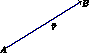
\includegraphics[scale=3.0]{vector.pdf}
   \caption{A Vector}
   \label{fig:figure-1-vector}
\end{figure}


\begin{eg}[Examples of vectors]
  Here are some important examples of vectors\\
  \vspace{-10px}
  \begin{itemize}
    \item The displacement of a particle is a vector.
    \item The velocity of a particle is a vector.
    \item The force acting on a particle is a vector.
  \end{itemize}

\end{eg}

\begin{notation}
  Vectors can be denoted in 3 ways,
  \begin{itemize}
    \item Using {\bf boldface notation}: $\boldsymbol{V}$
    \item Underlining:  $\underline{V}$ 
    \item An arrow over the symbol: $\vec{V}$

  \end{itemize}


\end{notation}

\section{Euclidean Three Space $\mathbb{E}^3$}

\begin{definition}[Euclidian Three Space]
 
  Euclidean Three Space is the set of all ordered triples of real numbers.\\
  \vspace{-10px}
  \begin{equation}
    \mathbb{E}^3 = \{(x,y,z) | x,y,z \in \mathbb{R}\}
  \end{equation}

\end{definition}

The \textbf{axes} of $\mathbb{E}^{3}$ are the $x$, $y$ and $z$, i.e.
\vspace{-10px}
\begin{equation}
  x = (x,0,0), y = (0,y,0), z = (0,0,z)
\end{equation}

We orient the axis according to the \textbf{right hand rule}. This is shown in the following diagram:

%generate tikz code for axes in 3d space

\begin{figure}[H]
  \centering
  \begin{tikzpicture}
    \draw[->] (0,0,0) -- (3,0,0) node[anchor=north east]{$y$};
    \draw[->] (0,0,0) -- (0,3,0) node[anchor=north west]{$z$};
    \draw[->] (0,0,0) -- (0,0,3) node[anchor=south]{$x$};
  \end{tikzpicture}
  \caption{Axes in $\mathbb{E}^3$}
\end{figure}

\begin{note}
  We need to pick an \textbf{origin} and stay with it. We will use the origin $(0,0,0)$.
\end{note} 

\section{Vectors in $\mathbb{E}^3$}
\subsection{Distance in $\mathbb{E}^3$}
Let $P$ and $P^{'}$ be points in $\mathbb{E}^3$. And let $P = (x,y,z)$ and $P^{'} = (x^{'},y^{'},z^{'})$.
\begin{definition}[Distance in $\mathbb{E}^3$]
  The \textbf{distance} between $P$ and $P^{'}$ is defined as:
  \begin{equation}
    d(P,P^{'}) = \sqrt{(x-x^{'})^2 + (y-y^{'})^2 + (z-z^{'})^2}
  \end{equation}
\end{definition}
This is illustrated in the following diagram
\begin{figure}[H]
\centering
   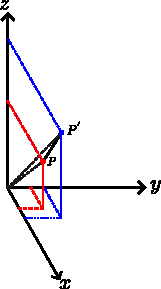
\includegraphics[scale=1.75]{distance.pdf}
   \caption{Distance in $\mathbb{E}^3$}
   \label{fig:figure-8-space}
\end{figure}
\clearpage
\subsection{Vectors in $\mathbb{E}^3$}
\begin{definition}[Vectors in $\mathbb{E}^3$]
  A \textbf{vector} in $\mathbb{E}^3$ is an ordered triple of real numbers.\\
  \vspace{-10px}
  \begin{equation}
    \vec{v} = (v_1,v_2,v_3)
  \end{equation}
\end{definition}

\begin{notation}
  We can also represent vectors using {\bf column notation}
  $$\underline{v} = \begin{bmatrix} v_1 \\ v_2 \\ v_3\end{bmatrix} $$
  
\end{notation}


\section{Vector Algebra}

\subsection{Vector Magnitude}

\begin{definition}[Vector Magnitude]
  Let $\vec{v} = (v_1, v_2, v_3)$ be a vector in $\mathbb{E}^3$. The \textbf{magnitude} of $\vec{v}$ is defined as:
  \begin{equation}
    \|\vec{v}\| = \sqrt{v_1^2 + v_2^2 + v_3^2}
  \end{equation}
\end{definition}

\subsection{Vector Addition}

\begin{definition}[Vector Addition]
  Let $\vec{v} = (v_1, v_2, v_3)$ and $\vec{w} = (w_1, w_2, w_3)$ be vectors in $\mathbb{E}^3$. The \textbf{sum} of $\vec{v}$ and $\vec{w}$ is defined as:
  \begin{equation}
    \vec{v} + \vec{w} = (v_1 + w_1, v_2 + w_2, v_3 + w_3)
  \end{equation}
\end{definition}

Geometrically this can be seen as the {\bf diagonal} of a paralleleogram. Geometrically it is clear that you get the same effect as travelling along $\vec{v}$ and then $\vec{u}$

\begin{figure}[H]
\centering
   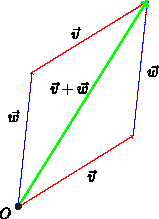
\includegraphics[scale=2.0]{vector_addition.pdf}
   \caption{Vector Addition} 
   \label{fig:figure-2-vector-addition}
\end{figure}

\clearpage

\subsubsection*{Vector Addition Properties}
\vspace{5px}
 
\begin{theorem}[Commutativity]
Suppose $\vec{v}$ and $\vec{w}$ be vectors in $\mathbb{E}^3$.\\
  If $\vec{v} = \left( v_1, v_2, v_3 \right)$ and $\vec{w} = \left(w_1, w_2, w_3 \right)$ be vectors in $\mathbb{E}^{3}$, then
  \begin{equation}
      \vec{v} + \vec{w} = \vec{w} + \vec{v}    
  \end{equation}
\end{theorem}
\begin{proof}
  
\end{proof}


\section{Standard Basis}
Standard basis vectors are also known as standard {\bf unit vectors}. These are used to represent vectors in $\mathbb{E}^3$

\begin{definition}
  The standard basis vectors are defined as follows:
  \begin{align*}
    \hat{i} &= (1, 0, 0 ) \\
    \hat{j} &=  (0, 1, 0) \\
    \hat{k} &=  (0, 0, 1)
  \end{align*}
such that $\mid \hat{i} \mid = \mid \hat{j} \mid = \mid \hat{k} \mid.$ 
\end{definition}

Any vector can be represented using standard basis vectors. 

Suppose you are a given a vector $\vec{v} = (v_1, v_2, v_3)$. This can be represented as follows:
\begin{equation}
  \vec{v} = \begin{bmatrix} v_1 \\ v_2 \\ v_3 \end{bmatrix}  =v_1\hat{i} + v_2\hat{j} + v_3\hat{k}
\end{equation}

\begin{eg}
  Let $\vec{v} = (2, 3, 4)$. Then, 
  \begin{align*}
    \vec{v} &= 2\hat{i} + 3\hat{j} + 4\hat{k} \\
    &= 2(1, 0, 0) + 3(0, 1, 0) + 4(0, 0, 1) \\
    &= (2, 0, 0) + (0, 3, 0) + (0, 0, 4) \\
    &= (2, 3, 4)
  \end{align*}
\end{eg}


\begin{figure}[H]
\centering
   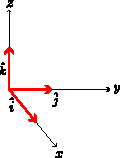
\includegraphics[scale=2.5]{standard-basis.pdf}
   \caption{Standard Basis Vectors}
   \label{fig:figure-3-unit-vector}
\end{figure}

\subsubsection{Algebra with Standard Basis Vectors}
\vspace{5px}
\begin{eg}
  Let $\vec{v}$ and $\vec{w} \in \mathbb{E}^3$ 
  \begin{flalign*}
    \vec{v} \pm \vec{w} = \begin{bmatrix} v_1 \pm w_1 \\ v_2 \pm w_2 \\ v_3 \pm w_3\end{bmatrix}  = (v_1 \pm w_1)\hat{i} + (v_2 \pm w_2)\hat{j} + (v_3 \pm w_3)\hat{k} &
  \end{flalign*}
\end{eg}


\begin{eg}
  Let $\vec{v}$ and $\vec{w} \in \mathbb{E}^3$ 
  \begin{flalign*}
    \lambda\vec{v} = \begin{bmatrix} \lambda v_1 \\ \lambda v_2 \\ \lambda v_3\end{bmatrix}  = (\lambda v_1)\hat{i} + (\lambda v_2)\hat{j} + (\lambda v_3)\hat{k} &
  \end{flalign*}
\end{eg}

\begin{note}
 The 0 vector is:
  $$\underline{0} = \begin{bmatrix} 0 \\ 0 \\ 0 \end{bmatrix} = 0\hat{i} + 0\hat{j} + 0\hat{k}$$
Any vector $\vec{v} \in \mathbb{E}^3$ added to the 0 vector is itself:
$$\vec{v} + \underline{0} = \vec{v}$$
\end{note}

Here is an example of algebra with standard basis vectors:
\begin{eg}
  Let $\vec{v} = (2, 3, 4)$ and $\vec{w} = (1, 2, 3)$. Then,
  \begin{align*}
    \vec{v} + \vec{w} &= (2, 3, 4) + (1, 2, 3) \\
    &= (2 + 1, 3 + 2, 4 + 3) \\
    &= (3, 5, 7)
  \end{align*}
\end{eg}

\subsubsection{Alternate Notation for Standard Basis Vectors}
\vspace{5px}
\begin{notation}
  We can change notation for standard basis vectors as follows:
  $$\hat{i} = \vec{e}_{1} \ \ \ \ \ \ \ \ \hat{j} = \vec{e}_{2} \ \ \ \ \ \ \ \ \hat{k} = \vec{e}_{3}$$
\end{notation}
and therefore we can write:
$$\vec{v} = v_1\hat{i} + v_2\hat{j} + v_3\hat{k} = \sum^{3}_{a=1}v_a \vec{e}_a$$

\section{Position Vectors}

\begin{definition}
  A {\bf position vector} is a vector that represents the position of a point in space relative to the origin, $O$. 
\end{definition}

Let any vector $\vec{v}$ be the position vector of a point $P$ in space. Then, the coordinates of $P$ are given by the components of $\vec{v}$:
\begin{figure}[H]
\centering
   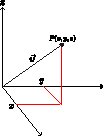
\includegraphics[scale=2.5]{position-vectors.pdf}
   \caption{Position Vector}
   \label{fig:figure-4-position-vector}
\end{figure}

So the position vector of $P$ is given by:
\begin{equation}
  \vec{v} = \begin{bmatrix} x \\ y \\ j \end{bmatrix}  =x\hat{i} + y\hat{j} + k\hat{k}
\end{equation}
\clearpage

\section{Scalar Product}

Scalar product is also known as dot product, is a function denoted by $\cdot$:
$$\cdot: \mathbb{E}^3 \times \mathbb{E}^3 \mapsto \mathbb{R}$$
i.e. it takes two vectors and returns a scalar.

\begin{definition}[Planar Angle]
  Let $\vec{v}$ and $\vec{w}$ be two vectors in $\mathbb{E}^3$ and $\theta \in \mathbb{R}$.
  \newline \newline
  The {\bf planar angle} between two vectors $\vec{v}$ and $\vec{w}$ is the angle $\theta$ between them in the plane spanned by $\vec{v}$ and $\vec{w}$.
  
  \begin{figure}[H]
    \centering
    \tikzset{every picture/.style={line width=0.75pt}} %set default line width to 0.75pt        

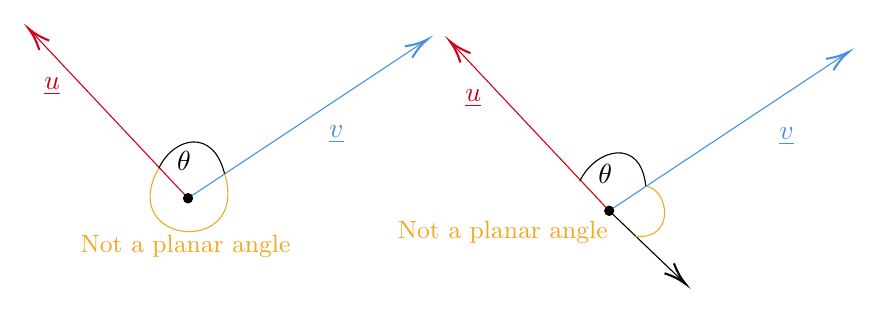
\begin{tikzpicture}[x=0.75pt,y=0.75pt,yscale=-1,xscale=1]
%uncomment if require: \path (0,402); %set diagram left start at 0, and has height of 402

%Straight Lines [id:da4437652617379132] 
\draw [color={rgb, 255:red, 208; green, 2; blue, 27 }  ,draw opacity=1 ]   (184.85,216.98) -- (109.47,136.76) ;
\draw [shift={(108.1,135.3)}, rotate = 46.79] [color={rgb, 255:red, 208; green, 2; blue, 27 }  ,draw opacity=1 ][line width=0.75]    (10.93,-3.29) .. controls (6.95,-1.4) and (3.31,-0.3) .. (0,0) .. controls (3.31,0.3) and (6.95,1.4) .. (10.93,3.29)   ;
%Straight Lines [id:da6919359366246228] 
\draw [color={rgb, 255:red, 74; green, 144; blue, 226 }  ,draw opacity=1 ]   (184.85,216.98) -- (298.51,141.58) ;
\draw [shift={(300.17,140.48)}, rotate = 146.44] [color={rgb, 255:red, 74; green, 144; blue, 226 }  ,draw opacity=1 ][line width=0.75]    (10.93,-3.29) .. controls (6.95,-1.4) and (3.31,-0.3) .. (0,0) .. controls (3.31,0.3) and (6.95,1.4) .. (10.93,3.29)   ;
%Shape: Ellipse [id:dp7599712014506931] 
\draw  [fill={rgb, 255:red, 0; green, 0; blue, 0 }  ,fill opacity=1 ] (182.67,216.98) .. controls (182.67,218.22) and (183.65,219.23) .. (184.85,219.23) .. controls (186.04,219.23) and (187.02,218.22) .. (187.02,216.98) .. controls (187.02,215.75) and (186.04,214.74) .. (184.85,214.74) .. controls (183.65,214.74) and (182.67,215.75) .. (182.67,216.98) -- cycle ;
%Curve Lines [id:da9435159136782311] 
\draw    (170.73,202.58) .. controls (178.25,187.05) and (197.1,183.3) .. (202.47,205.17) ;
%Curve Lines [id:da043732572464616704] 
\draw [color={rgb, 255:red, 245; green, 166; blue, 35 }  ,draw opacity=1 ]   (170.73,202.58) .. controls (149.85,239.67) and (214.99,245.71) .. (202.47,205.17) ;
%Straight Lines [id:da6201503651143601] 
\draw [color={rgb, 255:red, 208; green, 2; blue, 27 }  ,draw opacity=1 ]   (387.77,223.02) -- (312.4,142.8) ;
\draw [shift={(311.03,141.34)}, rotate = 46.79] [color={rgb, 255:red, 208; green, 2; blue, 27 }  ,draw opacity=1 ][line width=0.75]    (10.93,-3.29) .. controls (6.95,-1.4) and (3.31,-0.3) .. (0,0) .. controls (3.31,0.3) and (6.95,1.4) .. (10.93,3.29)   ;
%Straight Lines [id:da44499435743744065] 
\draw [color={rgb, 255:red, 74; green, 144; blue, 226 }  ,draw opacity=1 ]   (387.77,223.02) -- (501.43,147.62) ;
\draw [shift={(503.1,146.51)}, rotate = 146.44] [color={rgb, 255:red, 74; green, 144; blue, 226 }  ,draw opacity=1 ][line width=0.75]    (10.93,-3.29) .. controls (6.95,-1.4) and (3.31,-0.3) .. (0,0) .. controls (3.31,0.3) and (6.95,1.4) .. (10.93,3.29)   ;
%Shape: Ellipse [id:dp13145555074263104] 
\draw  [fill={rgb, 255:red, 0; green, 0; blue, 0 }  ,fill opacity=1 ] (385.6,223.02) .. controls (385.6,224.26) and (386.57,225.26) .. (387.77,225.26) .. controls (388.97,225.26) and (389.94,224.26) .. (389.94,223.02) .. controls (389.94,221.78) and (388.97,220.78) .. (387.77,220.78) .. controls (386.57,220.78) and (385.6,221.78) .. (385.6,223.02) -- cycle ;
%Curve Lines [id:da424029835736604] 
\draw    (373.66,208.62) .. controls (381.18,193.09) and (403.1,187.3) .. (405.39,211.2) ;
%Straight Lines [id:da38053982821885624] 
\draw    (387.77,223.02) -- (423.16,256.92) ;
\draw [shift={(424.6,258.3)}, rotate = 223.77] [color={rgb, 255:red, 0; green, 0; blue, 0 }  ][line width=0.75]    (10.93,-3.29) .. controls (6.95,-1.4) and (3.31,-0.3) .. (0,0) .. controls (3.31,0.3) and (6.95,1.4) .. (10.93,3.29)   ;
%Curve Lines [id:da7344761482411821] 
\draw [color={rgb, 255:red, 245; green, 166; blue, 35 }  ,draw opacity=1 ]   (405.39,211.2) .. controls (416.25,212.07) and (420.43,237.08) .. (400.38,235.36) ;

% Text Node
\draw (114.3,157.54) node [anchor=north west][inner sep=0.75pt]  [color={rgb, 255:red, 208; green, 2; blue, 27 }  ,opacity=1 ] [align=left] {$\displaystyle \underline{u}$};
% Text Node
\draw (251.61,180.86) node [anchor=north west][inner sep=0.75pt]  [color={rgb, 255:red, 74; green, 144; blue, 226 }  ,opacity=1 ] [align=left] {$\displaystyle \underline{v}$};
% Text Node
\draw (178.35,193.32) node [anchor=north west][inner sep=0.75pt]   [align=left] {$\displaystyle \theta $};
% Text Node
\draw (131.86,233.65) node [anchor=north west][inner sep=0.75pt]  [font=\small,color={rgb, 255:red, 245; green, 166; blue, 35 }  ,opacity=1 ] [align=left] {Not a planar angle};
% Text Node
\draw (317.22,163.58) node [anchor=north west][inner sep=0.75pt]  [color={rgb, 255:red, 208; green, 2; blue, 27 }  ,opacity=1 ] [align=left] {$\displaystyle \underline{u}$};
% Text Node
\draw (468.54,181.89) node [anchor=north west][inner sep=0.75pt]  [color={rgb, 255:red, 74; green, 144; blue, 226 }  ,opacity=1 ] [align=left] {$\displaystyle \underline{v}$};
% Text Node
\draw (381.28,199.36) node [anchor=north west][inner sep=0.75pt]   [align=left] {$\displaystyle \theta $};
% Text Node
\draw (284.68,226.75) node [anchor=north west][inner sep=0.75pt]  [font=\small,color={rgb, 255:red, 245; green, 166; blue, 35 }  ,opacity=1 ] [align=left] {Not a planar angle};

\end{tikzpicture}
\end{figure}

Choose the planar angle $\theta$ such that 
$$0 \leq \theta \leq \pi$$.
\end{definition}


\begin{definition}[Scalar Product]

  Let $\vec{v}$ and $\vec{w}$ be two vectors in $\mathbb{E}^3$ and $\theta \in \mathbb{R}$ be the planar angle between them. \\ 
Then, the scalar product of $\vec{v}$ and $\vec{w}$ is defined as:
  \begin{equation}
    \vec{v} \cdot \vec{w} = \mid \vec{v} \mid \mid \vec{w} \mid \cos \theta
  \end{equation}
\end{definition}

\begin{note}
  Two vectors do not lie in the same line, always in the same plane.
  By the convention, the angle $\theta \in [0,\pi] \Rightarrow 0 \leq \theta \leq \pi$.
\end{note}

\subsection{Properties of Scalar Product}
\begin{theorem}[Commutative]
Let $\vec{v}$ and $\vec{w}$ be two vectors in $\mathbb{E}^3$. Then,
  \begin{equation}
    \vec{v} \cdot \vec{w} = \vec{w} \cdot \vec{v}
  \end{equation}
\end{theorem}
\begin{proof}
Since the planar angle $\theta$ is the same for both $\vec{v}$ and $\vec{w}$,
\begin{align*}
  \vec{v} \cdot \vec{w} &= \mid \vec{v} \mid \mid \vec{w} \mid \cos \theta \\
  &= \mid \vec{w} \mid \mid \vec{v} \mid \cos \theta \\
  &= \vec{w} \cdot \vec{v}  
\end{align*}
\end{proof}
\begin{theorem}[Orthogonal Vectors]
 Let $\vec{v}$ and $\vec{w}$ be two vectors in $\mathbb{E}^3$. Then,
  \begin{equation}
    \vec{v} \cdot \vec{w} = 0 \iff \vec{v} \perp \vec{w}
  \end{equation} 
\end{theorem}
\begin{proof}
When $\vec{v} \perp \vec{w}$, the planar angle $\theta = \frac{\pi}{2}$. 
Therefore, 
\begin{align*}
  \vec{v} \cdot \vec{w} &= \mid \vec{v} \mid \mid \vec{w} \mid \cos \theta \\
  &= \mid \vec{v} \mid \mid \vec{w} \mid \cos \frac{\pi}{2} \\
  &= \mid \vec{v} \mid \mid \vec{w} \mid \cdot 0 \\
  &= 0
\end{align*}
  i.e. $\vec{v}$ and $\vec{w}$ are orthogonal.
\end{proof}

\begin{theorem}[Distributivity over scalar multiplication]
  Let $\vec{v}, \vec{w} \in \mathbb{E}^3$ and $\lambda \in \mathbb{R}$. Then,
  \begin{equation}
    \lambda(\vec{v} \cdot \vec{w}) = (\lambda \vec{v}) \cdot \vec{w} = \vec{v} \cdot (\lambda \vec{w})
  \end{equation}
\end{theorem}

\begin{theorem}[Distributivity over Addition]
  Let $\vec{u}, \vec{v}, \vec{w} \in \mathbb{E}^3$. Then,
  \begin{equation}
    \vec{u} \cdot (\vec{v} + \vec{w}) = \vec{u} \cdot \vec{v} + \vec{u} \cdot \vec{w}
  \end{equation}
\end{theorem}

\begin{note}
  Properties of scalar product for standard basis vectors:
  \begin{align*}
    \hat{i} \cdot \hat{i} &= 1 \\
    \hat{j} \cdot \hat{j} &= 1 \\
    \hat{k} \cdot \hat{k} &= 1 \\
    \hat{i} \cdot \hat{j} &= 0 \\
    \hat{i} \cdot \hat{k} &= 0 \\
    \hat{j} \cdot \hat{k} &= 0 \\
  \end{align*}
\end{note}

\subsection{Scalar Product in terms of Components}
\vspace{5px}
\begin{theorem}
  Let $\vec{v} = (v_1, v_2, v_3)$ and $\vec{w} = (w_1, w_2, w_3)$ be two vectors in $\mathbb{E}^3$. Then,
  \begin{equation}
    \vec{v} \cdot \vec{w} = \sum_{i=1}^{3}v_{i}w_{i} = v_1w_1 + v_2w_2 + v_3w_3
  \end{equation}
\end{theorem}
\begin{proof}
  Let $\vec{v}, \vec{w} \in \mathbb{E}^{3}$. Then, 
  \begin{flalign*}
    \vec{v} \cdot \vec{w} &= (v_1 \hat{i} + v_2 \hat{j} + v_3 \hat{k}) \cdot (w_1 \hat{i} + w_2 \hat{j} + w_3 \hat{k}) &\\ \\ 
      &= v_{1} \cdot (w_{1} \hat{i} + w_{2}\hat{j} + w_3 \hat{k}) + v_{2} \cdot (w_{1} \hat{i} + w_{2}\hat{j} + w_3 \hat{k}) + v_{3} \cdot (w_{1} \hat{i} + w_{2}\hat{j} + w_3 \hat{k})   &\\ \\
      &= v_{1}w_{1} \hat{i} \cdot \hat{i} + \cancel{v_{1}w_{2} \hat{i} \cdot \hat{j}} + \cancel{v_{1}w_{3} \hat{i} \cdot \hat{k}}  + \cancel{v_{2}w_{1} \hat{j} \cdot \hat{i}} + v_{2}w_{2} \hat{j} \cdot \hat{j} + \cancel{v_{2}w_{3} \hat{j} \cdot \hat{k}} \\  &+ \cancel{v_{3}w_{1} \hat{k} \cdot \hat{i}} + \cancel{v_{3}w_{2} \hat{k} \cdot \hat{j}} + v_{3}w_{3} \hat{k} \cdot \hat{k} &\\ \\
      &= v_{1}w_{1} + v_{2}w_{2} + v_{3}w_{3} &\\ \\ 
      &= \sum_{i=1}^{3}v_{i}w_{i} = v_1w_1 + v_2w_2 + v_3w_3
  \end{flalign*}
\end{proof}

\subsection{Using Scalar Product to find the length of a vector}
We can also use scalar product to find the length of a vector.
\begin{theorem}
  Let $\vec{v} \in \mathbb{E}^3$. Then,
  \begin{equation}
    \mid \vec{v} \mid = \sqrt{\vec{v} \cdot \vec{v}}
  \end{equation}
\end{theorem}
\begin{proof}
Let $\vec{v} \in \mathbb{E}^3$. Then,
  \begin{flalign*}
    \mid \vec{v} \mid &= \sqrt{v_1^{2} + v_2^{2} + v_3^{2}} \\ \\ 
    &= \sqrt{v_1v_1 + v_2v_2 + v_3v_3}  \\ \\
    &= \sqrt{\vec{v} \cdot \vec{v}}  
  \end{flalign*}
\end{proof}

\subsection{Using Scalar Product to find the angle between two vectors}

\begin{theorem}
  Let $\vec{v}, \vec{w} \in \mathbb{E}^3$. Then, the planar angle $\theta$ between $\vec{v}$ and $\vec{w}$ is given by:
  \begin{equation}
    \theta = \cos^{-1} \left( \frac{\vec{v} \cdot \vec{w}}{\mid \vec{v} \mid \mid \vec{w} \mid} \right)
  \end{equation}
\end{theorem}
\begin{proof}
  Let $\vec{v}, \vec{w} \in \mathbb{E}^3$. Then,
  \begin{flalign*}
    \vec{v} \cdot \vec{w} &= \mid \vec{v} \mid \mid \vec{w} \mid \cos \theta  \\ \\
    &= v_1w_1 + v_2w_2 + v_3w_3 \\ \\
    \Rightarrow \cos \theta &= \frac{v_1w_1 + v_2w_2 + v_3w_3}{\mid \vec{v} \mid \mid \vec{w} \mid} \\ \\
    \Rightarrow \theta &= \cos^{-1} \left( \frac{\vec{v} \cdot \vec{w}}{\mid \vec{v} \mid \mid \vec{w} \mid} \right)
  \end{flalign*}
\end{proof}

\begin{note}
  Some basic properties of scalar product:
  \begin{enumerate}
    \item If $\vec{v} \cdot \vec{w} = 0$, then $\theta = \frac{\pi}{2}$.
    \item If $\vec{v} \cdot \vec{w} > 0$, then $\theta \in [0, \frac{\pi}{2})$.
    \item If $\vec{v} \cdot \vec{w} < 0$, then $\theta \in (\frac{\pi}{2}, \pi]$.
  \end{enumerate}
\end{note}

\section{Cross Product}

\section{Kronecker-Delta}

As shown before, the properties of the {\bf scalar product}, the {\bf orthonormal basis} vectors have the following properties
$$\underline{e_{1}} \cdot \underline{e_{2}}= 0 = \underline{e_{1}} \cdot \underline{e_{3}} = \underline{e_{2}} \cdot \underline{e_{3}}$$
and
$$\underline{e_{1}} \cdot \underline{e_{1}}= 1 = \underline{e_{2}} \cdot \underline{e_{2}} = \underline{e_{3}} \cdot \underline{e_{3}}$$
We can abbreviate the definition using the {\bf Kronecker-Delta}

\begin{definition}[Kronecker-Delta]

	Let $a,b \in {1,2,3}$. Then we can write:

	\begin{equation}
		\label{eq:kronecker-delta}
		\underline{e_{a}}\cdot \underline{e_{b}}
		=
		\begin{cases}
			1 \ \ \text{if } a = b = 1,2,3 \\
			0  \ \ \text{if } a \neq b
		\end{cases}
		= \delta_{ab}
	\end{equation}

	This will also be useful for calculating scalar product
\end{definition}

\subsection{Scalar product using Kronecker-Delta}
\begin{theorem}[Scalar Product using Kroncker-Delta]
	Let $\vec{a} \vec{b} \in \mathbb{E}^3$. Then
	\begin{equation}
		\vec{a} \cdot \vec{v} = \sum_{i=1}^{3}a_kb_k
	\end{equation}
\end{theorem}
\begin{proof}
	\begin{align*}
		\underline{a} \ \cdot \ \underline{b} & = \Big( \sum\limits_{k = 1}^{3}a_k\underline{e_{k}} \Big)\ \cdot \ \Big( \sum\limits_{l = 1}^{3}b_l\underline{e_{l}} \Big) \\ \\
		                                      & = \sum_{k, \ l} a_{k} \ b_{l} \ \underline{e_{k}}\ \cdot \ \underline{e_{l}}                                               \\ \\
		                                      & = \sum_{k, \ l} a_{k} \ b_{l} \ \delta_{kl}
	\end{align*}
	Now by the definition of Kronecker-Delta \ref{eq:kronecker-delta}, it is 0 for all cases except when $k = l$. where it has a value of {\bf 1} So the summation becomes:
	$$\underline{a} \ \cdot \underline{b} =\sum_{k=1}^{3} a_{k} \ b_{k}$$
\end{proof}

\section{Levi-Civita}
We can represent the cross product using {\bf Levi-Civita Symbol}

\begin{definition}[Levi-Civita]
	Let $a, b, c \in {1,2,3}$. Then we write:
	\begin{equation}
		\label{eq:levi-civita}
		\varepsilon_{abc}
		=
		\begin{cases}
			0  \ \ \ \ \  \text{if } \space a = b = c  \space \space \text{ or more generally} \space a,b,c \space \text{is {\bf not} permutation of } \space 1,2,3 \\
			+1  \ \ \ \ \  \text{if } \space a,b,c \space \text{ is an {\bf even} permuation of } \space 1,2,3                                                      \\
			-1  \ \ \ \ \ \text{if } \space a,b,c \space \text{ is an {\bf odd} permuation of } \space 1,2,3
		\end{cases}
	\end{equation}
\end{definition}

\begin{note}
	Value of $\varepsilon_{abc}$ depends on the {\bf parity} of the permutatiom.
\end{note}

\subsection{Cross product of Orthonoarmal Basis Using Levi-Civita}
\begin{definition}
	Then we can write the cross product {\bf Orthonoarmal Basis Vectors} $\underline{e_1}, \underline{e_2}, \underline{e_3}$ in the following way
	\begin{equation}
		\label{eq: levi-orthonormal}
		\underline{e_a} \times \underline{e_b} = \sum_{i=1}^{3}a_{k}b_{k}\varepsilon_{abc}
	\end{equation}

\end{definition}

\subsection{Cross Product of Vectors in Levi-Civita Notation}
\begin{theorem}[Cross Product using Levi-Civita Notation]
	Let $\vec{a}, \vec{b} \in \mathbb{E}^3$. Then
	\begin{equation}
		\label{eq:levi-civita-cross-product}
		\vec{a} \times \vec{b} = \sum_{m=1}^{3}(\vec{a} \times \vec{b})_{m}\underline{e_m}
	\end{equation}
	where $(\vec{a} \times \vec{b})_m$ is the {\bf mth component}
	\begin{equation}
		\label{eq: mth-component}
		(\vec{a} \times \vec{b})_m = \sum_{k, \ l}\varepsilon_{abc}a_{k}b_{l}
	\end{equation}
\end{theorem}
\begin{proof}
	Let
	$$
		\underline{a} = a_{k}\underline{e_{k}} = \sum_{k=1}^{3}a_{k}\ \underline{e_{k}} \hspace{100px} \underline{b} = b_{l}\underline{e_{l}}= \sum\limits_{l=1}^{3} b_{l}\ \underline{e_{l}}
	$$
	Observe the use of {\bf Eintein's Notation} (see below) and observe that
	\begin{align*}
		\underline{a} \times \underline{b} & = \Big( \sum\limits_{k = 1}^{3}a_k\underline{e_{k}} \Big)\ \times \ \Big( \sum\limits_{l = 1}^{3}b_l\underline{e_{l}} \Big) \\ \\
		                                   & = \sum\limits_{k, \ l}a_{k} \ b_{k} \ \underline{e_{k}} \times \underline{e_{l}}
	\end{align*}
	And therefore by \ref{eq: levi-orthonormal}, we can rewrite it in the following way
	$$\hspace{-80px} = \sum\limits_{k,\ l,\ m} a_{k} \ b_{l} \ \epsilon_{klm} \ \underline{e_m}$$
	Define the {\bf mth component} as
	$$(\vec{a} \times \vec{b})_m =  \sum_{k, \ l}\varepsilon_{abc}a_{k}b_{l}$$
	and hence we get \ref{eq:levi-civita-cross-product}
\end{proof}

\section{Einstein's Notation}

\begin{definition}[Einstein's Notation]

	If {\bf two} indicies are {\bf repeated}, then they are {\bf summed} and we can {\bf suppress} the summation
\end{definition}

\subsection{Scalar Product using Einstein Convention}
\begin{eg}
	$$\sum_{i=1}^{3}a_{k}b_{k} = a_{k}b_{k}$$
	Here the {\bf repeated index} is $k$
\end{eg}

\subsection{Cross Product using Einstein Convention}
\begin{eg}
	Here the {\bf repeated index} is $k$ and $l$
	$$(a \ \times\ b)_{m}= \sum\limits_{k,\  l}^{3}\epsilon_{klm}a_{k}\ b_k =\epsilon_{klm} a_{k} \ b_{k}$$

\end{eg}

\section{Triple Scalar Product}

\begin{theorem}[Triple Scalar Product]
	Let $\vec{a}, \vec{b}, \vec{c} \in \mathbb{E}^{3}$. Then
	\begin{equation}
		\label{eq: triple-scalar-product}
		\vec{a} \cdot (\vec{b} \times \vec{c}) = \varepsilon_{abc}a_pb_qc_r
	\end{equation}
\end{theorem}
\begin{note}
	We have used \textbf{Einstein's Notation} for Scalar and Vector Product as well as Levi-Civita Notation \ref{eq:levi-civita}
\end{note}
\begin{proof}
	\begin{align*} \underline{a} \ \cdot \ (\underline{b} \times \underline{c}) & = a_{p}\ (\underline{b} \times \underline{c})_{p} \\ \\ &= a_{p}\ \epsilon_{pqr}\ b_{q}\ c_{r}\\ \\
                                                                            & = \epsilon_{pqr}\ a_{p}\ b_{q}\ c_{r}\end{align*}
\end{proof}
\begin{note}
	Although not mathematically valid, we can use the {\bf determinant method}
	$$\underline{a} \cdot(\underline{b} \times \underline{c}) =
		\det\begin{pmatrix}a_1 & a_2 & a_3 \\ b_{1} & b_{2} & b_{3} \\ c_{1}  & c_{2} & c_{3}\end{pmatrix}$$
\end{note}

\section{Useful Properties of Kronecker-Delta and Levi-Civita}
\begin{theorem}
	\begin{equation}
		\label{eq: levi-kronecker-property-1}
		\epsilon_{pqr}\epsilon_{ruv} = (\delta_{pu}\delta_{qv} - \delta_{pv}\delta_{qu})
	\end{equation}
\end{theorem}
\begin{note}
	These are useful identity/trick to remember (remeber the use of {\bf Einstein's Notation})
	$$\delta_{aa} = \delta_{11} + \delta_{22} + \delta_{33} = 3$$
	\\
	\begin{equation*}
		\delta_{ab}\delta_{bc}=\delta_{a1}\delta_{1c} + \delta_{a2}\delta_{2c} + \delta_{a3}\delta_{3c}
		= \begin{cases}
			1 & \text{if } a = c    \\
			0 & \text{if } a \neq c
		\end{cases}
		\ \ \ = \delta_{ac}
	\end{equation*}
\end{note}


\section{Triple Vector Product}
\begin{theorem}[Triple Vector Product]
	Let $\underline{a}, \underline{b}, \underline{c} \in \mathbb{E}^3$
	\begin{equation}
		\label{eq: triple-vector-product}
		\underline{a} \times (\underline{b} \times \underline{c}) = \underline{b}(\underline{a} \cdot \underline{c}) - \underline{c}(\underline{a} \cdot \underline{b})
	\end{equation}
\end{theorem}
\begin{proof}
	Taking three vectors $\underline{a}, \underline{b} \text{ and } \underline{c}$, we {\em calculate} the \textbf{pth component} first:
	\begin{align*}
		[\underline{a} \times (\underline{b} \times \underline{c})]_{p} & = \epsilon_{pqr}\ a_{q}(\underline{b} \times \underline{c})_{r} \\ \\
		                                                                & = \epsilon_{pqr}\ a_{q} \ \epsilon_{ruv}\ b_{u}\ c_{v}
	\end{align*}
	using identity \ref{eq: levi-kronecker-property-1}, we get
	\begin{align*}
		[\underline{a} \times (\underline{b} \times \underline{c})]_{p} & = (\delta_{pu}\delta_{qv} - \delta_{pv}\delta_{qu})a_{q}b_{u}c_{v}
	\end{align*}
	Use the explanation below for completion
\end{proof}

\begin{figure}[H]
	\centering
	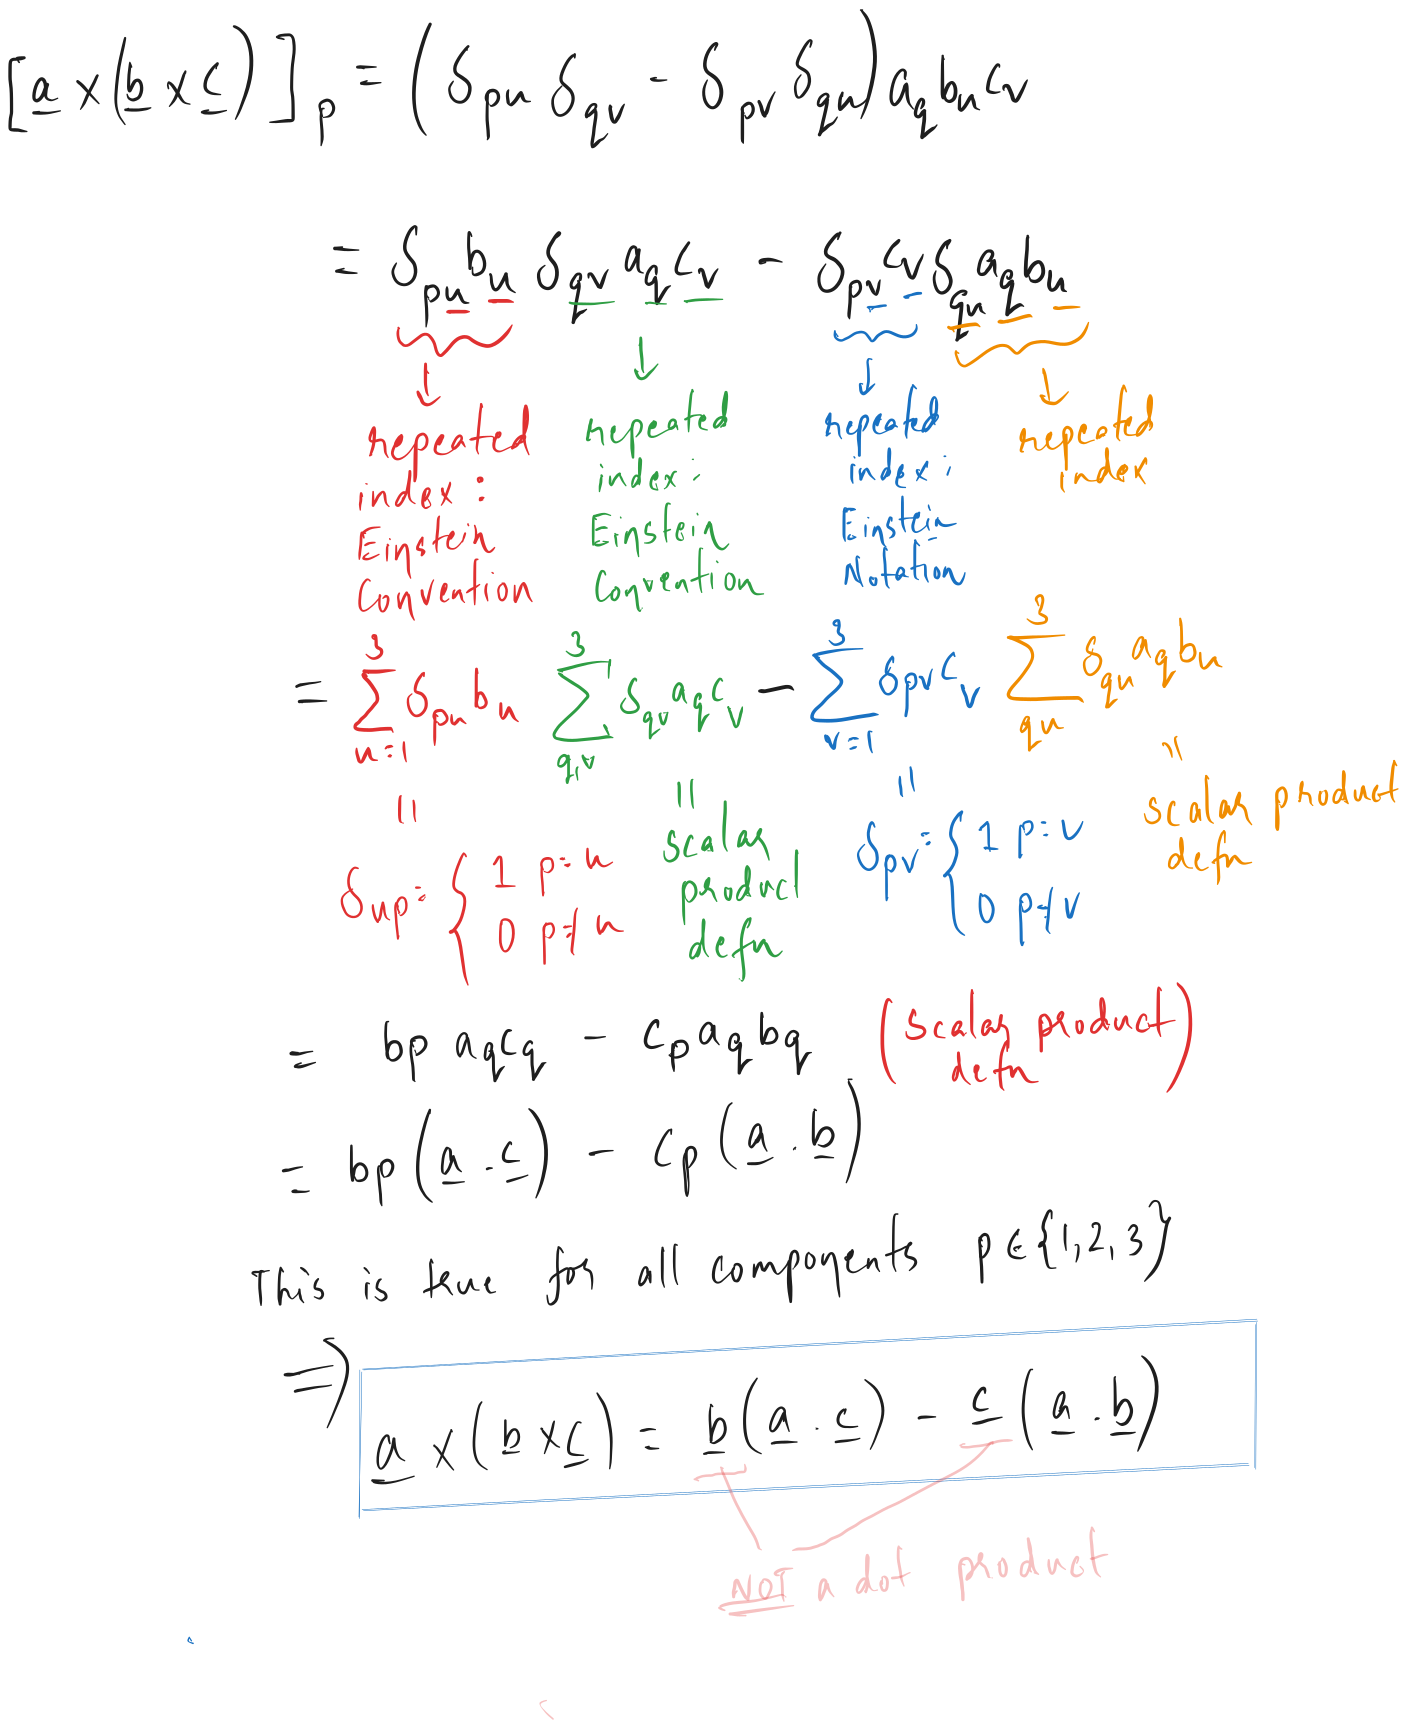
\includegraphics[scale=0.35]{triple-vector-product-proof.png}
	\caption{Triple Vector Product Proof}
	\label{fig:figure-triple-vector-product-proof}
\end{figure}

\clearpage

% end lectures
\end{document}
